\section{Lecture 10 - 09/28/2022}

Clarification from last lecture: In the proof of the Casorati–Weierstrass theorem, we have that $g(z) \neq 0$ for all $z \in U\setminus \{z_0\}$, but $g(z_0) = 0$ is totally possible! Hence we write
\[f(z) = \frac{1}{g(z)} + a\]
, where $f$ either has a pole or a removable singularity at $z_0$, giving the contradiction.

\subsection{Computing Real Integrals with Residues}

\begin{example}[A Straight-forward Application]
Let $s \in \Rbb$, consider the integral
\[I = \int_{-\infty}^\infty \frac{1}{x^2 + 1} e^{isx} dx\]
Let $f(z) = \frac{1}{x^2 + 1} e^{isx}$, then $I = \int_{\Rbb} f(z) dz = \pi e^{-|s|}$
\end{example}

\begin{remark}
Why do we even care about integrals of this form? Well, they are really closed aligned with \textbf{inverse Fourier transforms}. In particular, you would calculate integrals of the form
\[F(s) = \int_{-\infty}^\infty f(x) e^{-2\pi i s} dx\]
\end{remark}

\begin{proof}[Proof of Example]
We will consider three cases $s = 0, s > 0,$ and $s < 0$. For $s = 0$, this is obvious.\\\\
Now for $s > 0$, consider the following contour:
\[\fbox{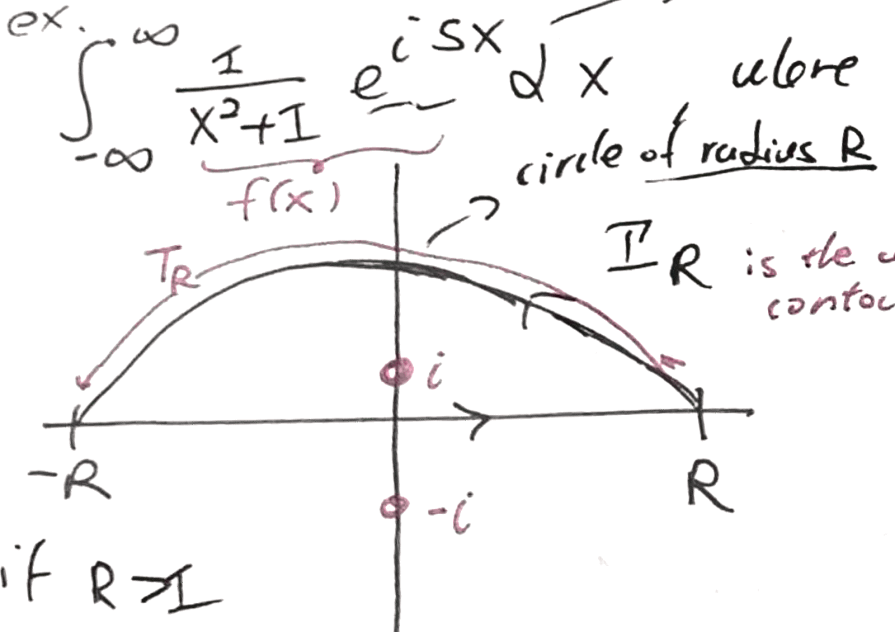
\includegraphics[width=.5\textwidth]{Figures/contour-1.png}}\]
Then Cauchy's Residue Theorem tells us that
\[\int_{\Gamma_R} f(z) dz = 2 \pi i Res(f, i)\]
$i$ is a pole of order $1$ for $f$, so
\[Res(f, i) = \lim_{z \to i} (z -i)f(z) = \frac{e^{-s}}{2i}\]
Thus, we have that
\[\int_{\Gamma_R} f(z) dz = \pi e^{-s}\]
Now take $R \to \infty$, we note that since \textbf{$f$ is integrable} as $\int_{-\infty}^\infty |f(x)| dx < \infty$,
\[\lim_{R \to \infty} \int_{-R}^R f(z) dz = \int_{-\infty}^{\infty} f(z) dz = I\]
So in other words,
\[I = \lim_{R \to \infty} [\int_{\Gamma_R} f(z) dz - \int_{T_R} f(z) dz] = \pi e^{-s} - \lim_{R \to \infty} \int_{T_R} f(z) dz\]
We want to show that the last term goes to $0$, indeed
\begin{align*}
    \int_{T_R} f(z) dz &= \int_0^\pi \frac{e^{isRe^{it}}}{(Re^{it})^2 + 1} i Re^{it} dt \tag*{Let $z = R e^{it}$}\\
    |\int_{T_R} f(z) dz| &\leq \frac{R}{R^2 - 1} \pi \tag*{Note that $e^{isRe^{it}}$ is bounded by $1$ as $s > 0$ and $0 < t < \pi$}
\end{align*}
Taking $R \to \infty$, the bound goes to $0$, thus, we have that
\[I = \pi e^{-s}, s \geq 0\]
\textbf{What about when $s < 0$}? In this case, $\int_{T_R} f(z) dz$ would not actually go to $0$, so instead, we need to consider the opposite contour:
\[\fbox{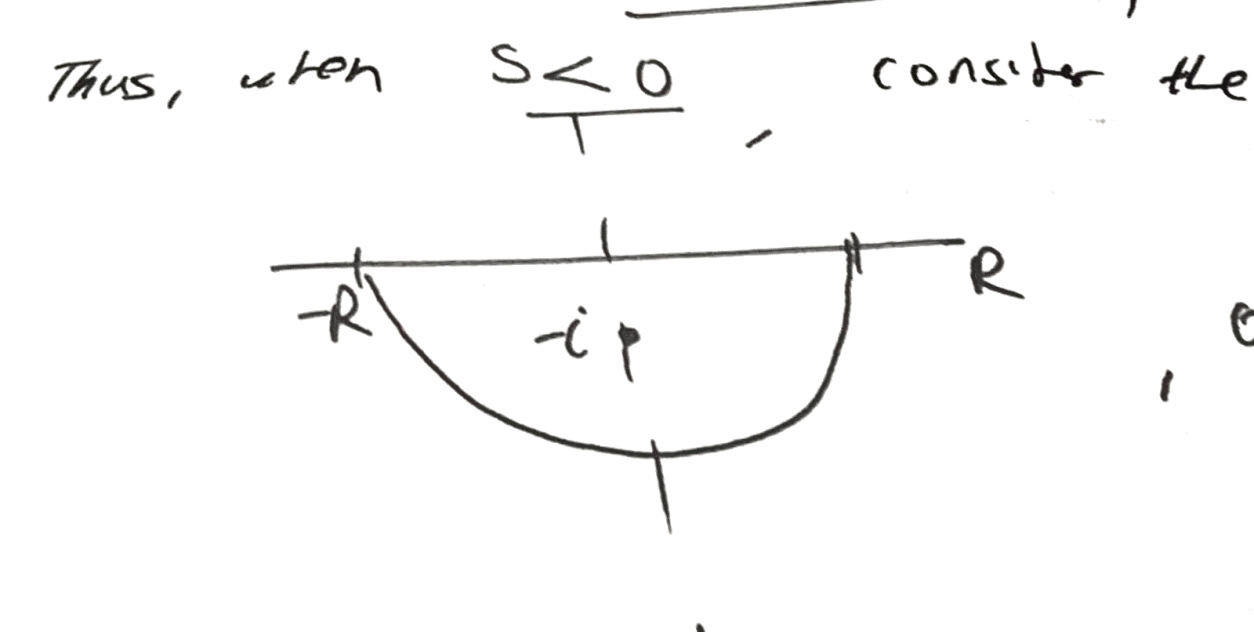
\includegraphics[width=.5\textwidth]{Figures/contour-2.png}}\]
, and we can similarly show the result is true. Alternatively, we could also have argued using symmetry.\\\\
Note that while we proved this using a circle, we could have also used a rectangle instead.
\end{proof}

\begin{example}[A Not-So-Simple Application]
Let $s \in \Rbb$ and $a \in \Cbb$ such that $s > 0$ and $\Im(a) > 0$, consider the integral
\[I = \int_{-\infty}^\infty \frac{e^{isx}}{x - a} dx\]
Let $f(z) = \frac{e^{isz}}{z - a}$, then what is $I$?
\end{example}

Consider the following contour:
\[\fbox{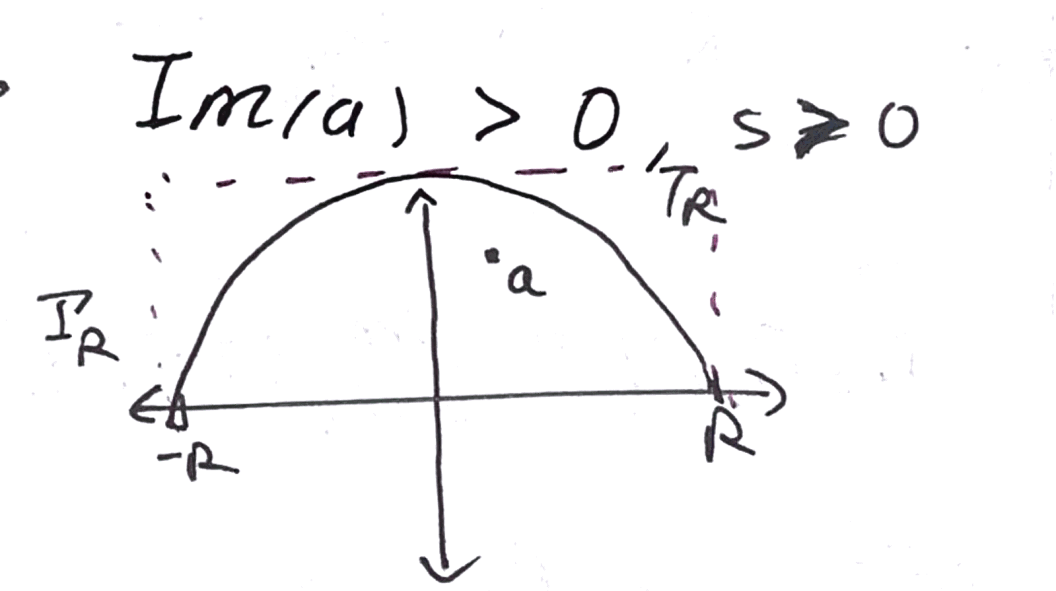
\includegraphics[width=.5\textwidth]{Figures/contour-3.png}}\]
where $R > |a|$, while we could use a rectangle, we will stick with the half-circle again. Then again Cauchys' Residue Theorem tells us that
\[\int_{\Gamma_R} f(z) dz = 2\pi i Res(f, a)\]
$a$ is a pole of order $1$ of $f$, so we have that
\[Res(f, a) = \lim_{z \to a} (z - a) \frac{e^{isz}}{z - a} = e^{isa}\]
However, we note that $f$ is actually \textbf{NOT INTEGRABLE}, so the following limit need not exist
\[\lim_{R \to \infty} \int_{-R}^R f(x) dx\]
Howebver, if $\int_{T_R} f(z) dz = 0$, then the limit would exist, and we would have
\[\lim_{R \to \infty} \int_{-R}^R f(x) dx = 2 \pi i e^{isa} = p.v \int_{-\infty}^\infty f(x) dx\]
However, we run into a problem with doing $ML$-esitmate on $\int_{T_R} f(z) dz = 0$, because it turns out it'd give us
\[|\int_{T_R} f(z) dz| \leq \frac{R}{R - |a|} \pi \]
, which does not converge to $0$ as $R \to \infty$.\\

Fortunately, we do have a workaround:
\begin{lemma}[Jordan's Lemma]
Let $C \in \Rbb$ be some fixed constant, then
\[\int_{T_R} |e^{iz}| |dz| \leq C\]
, where $|dz|$ is with respect to the Lebesgue Measure of the unit circle.
\end{lemma}

Now take $z = R e^{i \theta}$, then $dz = i R e^{i \theta} d \theta$, so we have that $|dz| = R |d \theta|$.

\begin{corollary}
If $s > 0$, then 
\[\int_{T_R} |e^{iz}| |dz| \leq C(s)\]
, where $C(s)$ is some constant dependent on $s$.
\end{corollary}

\begin{remark}
Jordan's Lemma for circles are generally hard to show, so most textbooks only prove it on a rectangle instead:
\[\fbox{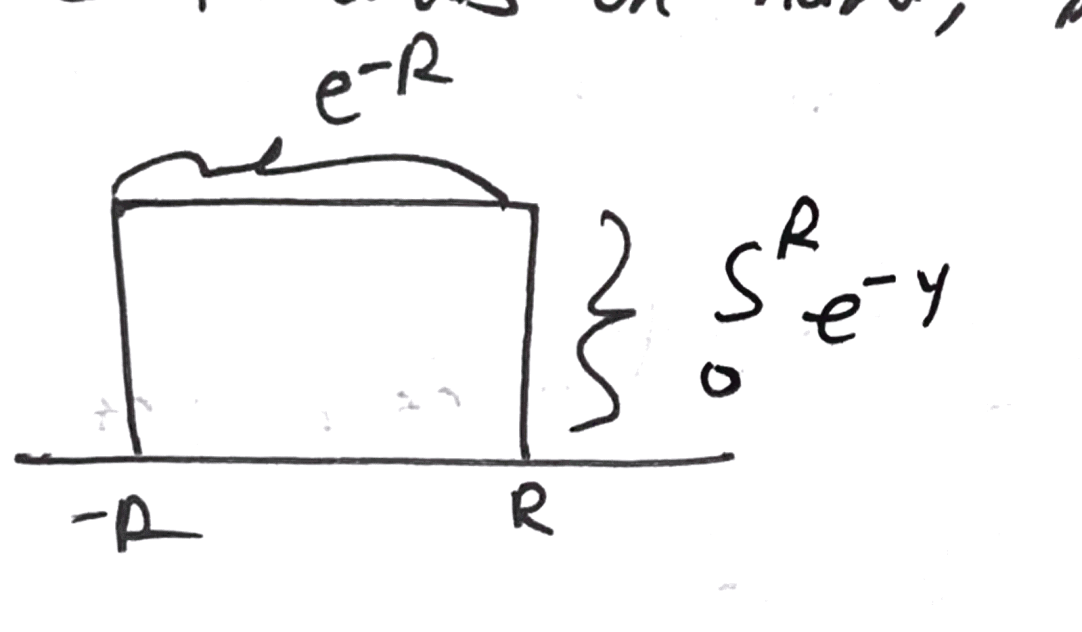
\includegraphics[width=.5\textwidth]{Figures/contour-4.png}}\]
\end{remark}

Now, using Jordan's Lemma, we have that
\begin{align*}
    |\int_{T_R} \frac{e^{isz}}{z - a} dz| &\leq \frac{1}{R - |a|} \cdot \int_{T_R} |e^{isz}| |dz|\\
    &\leq \frac{C(s)}{R - |a|}
\end{align*}
, so the limit goes to $0$ as $R \to \infty$.

\begin{question}
What about if $\Im(a) < 0$ and $s > 0$?
\end{question}

 In this case, we can either close the lower half or use a change of variables to get the same result.

\begin{question}
What about if $\Im(a) > 0$ but $s < 0$?
\end{question}

In this case, we will consider the contour
\[\fbox{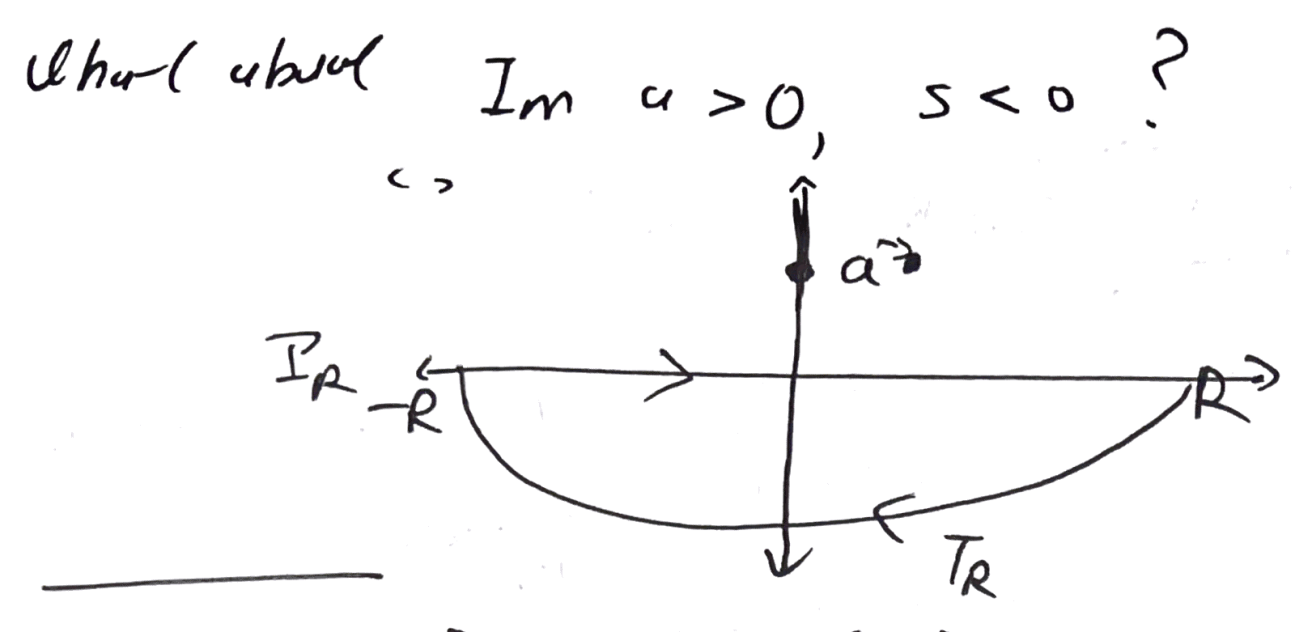
\includegraphics[width=.5\textwidth]{Figures/contour-5.png}}\]
There are no singularities inside the contour so
\[\int_{\Gamma_R} f(z) dz = 0\]
In addition, as $R \to \infty$, we also have that
\[\int_{T_R} f(z) dz = 0\]
Thus, the integral $I$ is just $0$.

\begin{question}
What if $a \in \Rbb \setminus \{0\}$ and $s > 0$?
\end{question}

In this case, consider the contour:
\[\fbox{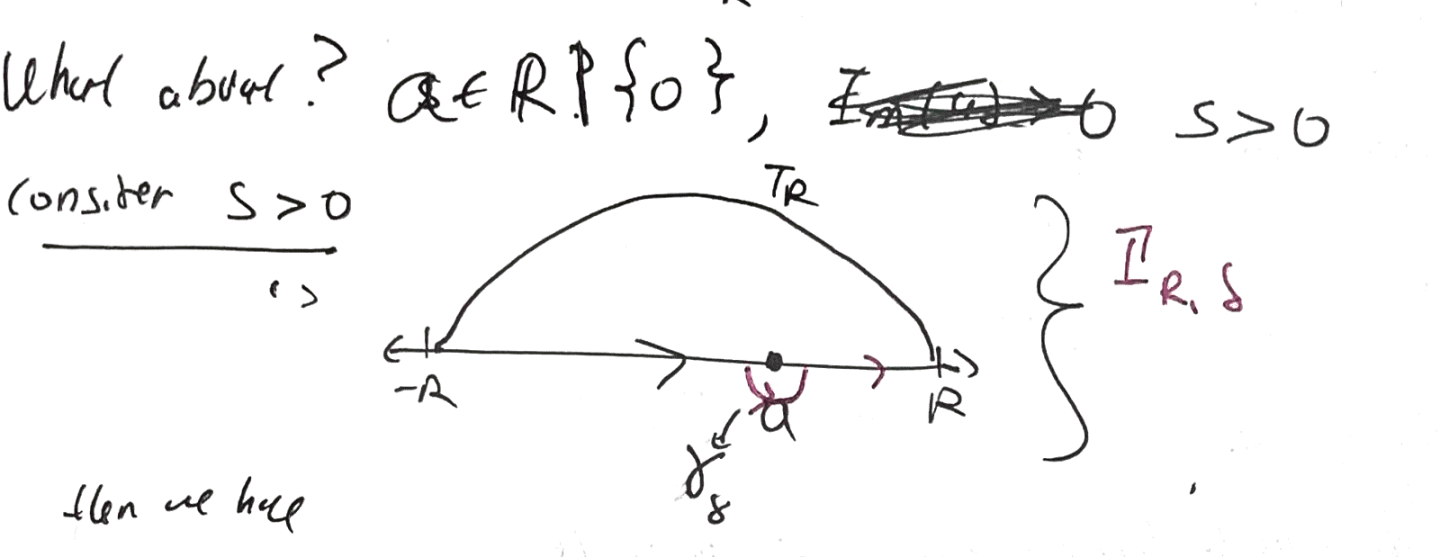
\includegraphics[width=.5\textwidth]{Figures/contour-6.png}}\]

In this, case we note that as we expand $R$ and shrink $\delta$, we have that
\[\int_{[-R, R] \setminus [a - \delta, a + \delta]} \mapsto p.v \int_{-\infty}^\infty f(z) dz\]

Cauchy's Residue Theorem tells us that
\[\int_{\Gamma_{R, \delta}} f(z) dz = 2 \pi i Res(f, a) = 2 \pi i e^{isa}\]

Jordan's Lemma tells us that
\[\lim_{R \to \infty} \int_{T_R} f(z) dz = 0 \]

Finally, taking $\delta \to 0$ gives that
\[\int_{\gamma_\delta} f(z) dz = \pi i e^{isa}\]

Thus, we have that
\[p.v \int_{-\infty}^\infty f(z) dz = 2 \pi i e^{isa} - \pi i e^{isa} = \pi i e^{isa}\]